\section{Connection}\label{sec:testconnection}
% introduktion
I følgende afsnit er beskrevet hvordan test og integration er foretaget for connection delen. Denne del integrerer både med databasen og applikationen, samt intern integration mellem 2 kørende applikationer i form af en TCP/IP socket forbindelse.

\subsection{Testdetaljer}
% beskrivelse af coverage procent og antallet af test, samt begrundelse for begge.
I connection delen har der været mest fokus på, at lave unit tests til de interne systemer, som Token systemet og generering af pool data. Årsagen til dette, er at de andre klasser er relativt simple i sig selv, og derfor primært er blevet integrationstestet, hvilket er foregået via manuel test med de andre projekt dele. De kørte unittests er vist på figur~\ref{fig:connectionunittest}

% BILLEDE AF KØRTE UNITTEST
\begin{figure}[H]
	\centering
	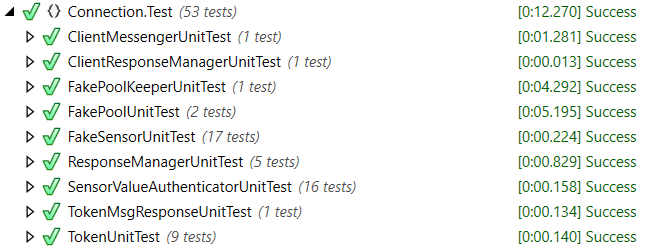
\includegraphics[width=0.9\linewidth]{figs/connection/unittest.png}
	\caption{Unittest af connection.}
	\label{fig:connectionunittest}
\end{figure}
% BILLEDE AF COVERAGE KØRT

De kørte unittests giver en relativt lav coverage. Dette skyldes at hele message systemet, som ligger i Connection.Model, består af en lang række klasser uden adfærd, og derfor ikke er testet. Socket klient og server er desuden ikke testet, og er derfor excluderet fra coverage. Dette skyldes at de er implementeret udfra eksempler givet på msdn.com ??. Samlet giver dette en coverage på 73\% som vist på figur~\ref{fig:connectioncoverage}

\begin{figure}[H]
	\centering
	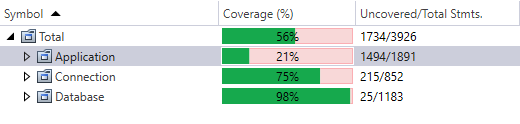
\includegraphics[width=0.9\linewidth]{figs/connection/coverage.png}
	\caption{Coverage af connection}
	\label{fig:connectioncoverage}
\end{figure}

\subsection{Testbeskrivelse}
% hvordan div. test er valgt og hvad I specielt var opmærksom på under udviklign af test. 
% hvad var let/svært at teste etc.
Tests er opbygget udfra metoder, hvor der for hver metode er testet de forskellige mulige gennemløb af metoden. Udfra dette, skulle der i teorien gerne opnås en coverage på 100\%. Dette kan ses på figur~\ref{fig:pooldatatest} hvor der er vist tests af de klasser som tilsammen udgør generering af pool data. Årsagen til at der her ikke er 100\% coverage, er metoder der indeholder en switch-case med et enum. Dette medfører at default ikke bliver eksekveret, og ikke kan fakes uden at ændre på den nuværende enum, hvilket ikke ønskes. 
\begin{figure}[H]
	\centering
	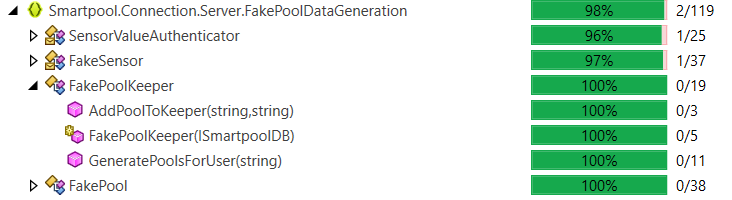
\includegraphics[width=0.9\linewidth]{figs/connection/pooldatatest.png}
	\caption{Unittest af pool data generering}
	\label{fig:pooldatatest}
\end{figure}